\documentclass{article}
\usepackage{latexsym}
\usepackage{amssymb,amsmath}
\usepackage{custom2}
\usepackage{graphicx} % for figures
\usepackage{epstopdf} % so can use EPS or PDF figures
\usepackage{subfig}
\usepackage{url}
\usepackage{amssymb,amsfonts}
\usepackage[all,arc]{xy}
\usepackage{enumerate}
\usepackage{mathrsfs}
\usepackage{booktabs}
\usepackage[pdftex]{hyperref}
\usepackage{lscape}
\captionsetup{justification=RaggedRight, singlelinecheck=false}
\newcommand{\ra}[1]{\renewcommand{\arraystretch}{#1}}
\newcommand{\argmax}{\text{argmax}}
\newcommand{\Tr}{\text{Tr}}
%\newtheorem{claim}{Claim}

\addtolength{\evensidemargin}{-.5in}
\addtolength{\oddsidemargin}{-.5in}
\addtolength{\textwidth}{1.4in}
\addtolength{\textheight}{1.4in}
\addtolength{\topmargin}{-.5in}

\pagestyle{empty}

\begin{document}
\begin{center}
\Large

\end{center}


\vspace{0pt}

\begin{center}
{\bf \LARGE{Evolution of Topological Strategies}}
\vspace{10pt}
\\ Eleanor Brush
\\ August 28, 2012
\end{center}

\vspace{0pt}
\normalsize

\section{Linear Algebra Preliminaries}

\begin{claim}
Let $v\in\R^n\setminus\{0\}$.  Let $A\in\R^{n-1\times n}$ be such that the rows of $A$ are an orthonormal basis to the orthogonal complement of $v$.  Then $A^TA=I_n-\frac{1}{||v||^2}vv^T$ (where $v$ is $v$ as a column vector so that $v\times v^T\in\R^{n\times n}$).
\end{claim}

\begin{pf}
Let $\tilde{v}$ and let $V=\left[\begin{array}{cc}A \\ \tilde{v}^T\end{array}\right].$  Then $V\in\R^{n\times n}$ and by construction the rows of $V$ are an orthonormal basis for $\R^n$.  First, we argue that $V^TV=I_n:$
\begin{align*}
V^TV&=M
\\ \Rightarrow VV^TV&=VM
\\ \Rightarrow V&=VM \text{ since the rows of $V$ are orthonormal} 
\\ \Rightarrow M&=I_n \text{ since $V$ is nonsingular}
\end{align*}
Then,
\begin{align*}
V^TV&=\left[A^T \tilde{v}\right]\times\left[ \begin{array}{cc}A\\ \tilde{v}^T\end{array}\right]
\\\Rightarrow (V_T^V)_{ij}&=\sum_kA_{ki}A_{kj}+v_iv_j \text{ for all $i,j$}
\\ \Rightarrow (V_TV)_{ij}&=(A^TA)_{ij}+(\tilde{v}\tilde{v}^T)_{ij} \text{ for all $i,j$}
\\ \Rightarrow V_TV&=A^TA+\tilde{v}\tilde{v^T}
\\ \Rightarrow A^TA&=V_TV-\tilde{v}\tilde{v^T}
\\ \Rightarrow A^TA&=I_n-\frac{1}{||v||^2}vv^T
\end{align*}
\end{pf}

\begin{claim}
Let $B\in\R^{n\times n}$ and $v$ be an eigenvector of $B$ with associated eigenvalue $\lambda$.  Let $A\in\R^{n-1\times n}$ be such that the rows of $A$ are an orthonormal basis to the orthogonal complement of $v$.  Then $\sigma(ABA^T)=\sigma(B)\setminus\{\lambda\}$ (where $\sigma(M)$ is the spectrum of $M$, i.e. the set of eigenvalues of $M$, with each eigenvalue appearing as many times as its algebraic multiplicity).
\end{claim}

\begin{pf}
Let $\tilde{v}=\frac{v}{||v||}$ and let $V=\left[\begin{array}{cc}A \\ \tilde{v}^T\end{array}\right].$  Since $V$ is orthonormal, $VBV^T$ has the same eigenvalues as $B$.
\begin{align*}
VBV^T&=\left[\begin{array}{cc}A \\ \tilde{v}^T\end{array}\right]\times B\times \left[A^T\tilde{v}\right]
\\&=\left[\begin{array}{cc} ABA^T & AB\tilde{v} \\ \tilde{v}^TBA^T & \tilde{v}^TB\tilde{v} \end{array}\right]
\\&=\left[\begin{array}{cc} ABA^T & \lambda A\tilde{v} \\ \tilde{v}^TBA^T & \lambda \tilde{v}^T\tilde{v} \end{array}\right]
\\&=\left[\begin{array}{cc} ABA^T & 0 \\ \tilde{v}^TBA^T & \lambda  \end{array}\right] \text{ by construction of $A$}
\end{align*}
Therefore, the eigenvalues of $VBV^T$ are the eigenvalues of $ABA^T$ and $\lambda$.  But, as noted above, the eigenvalues of $VBV^T$ are the same as the eigenvalues of $B$.  Therefore, $\sigma(ABA^T)=\sigma(B)\setminus\{\lambda\}$ (where $\sigma(M)$ includes each eigenvalue as many times as its algebraic multiplicity).
\end{pf}

\begin{claim}
Let $M\in\R^{n\times n}$ with eigenvalues $\lambda_1\geq\lambda_2\dots\geq\lambda_n$ and associated eigenvectors $u_1,\dots,u_n$.  Let $v\in\R^n$.  Let $u_i$ be the eigenvector such that 
$$i=\argmax_j\left\{\left\langle \frac{v}{||v||},\frac{u_j}{||u_j||}\right\rangle \right\}.$$
Let $A\in\R^{n-1\times n}$ be such that the rows of $A$ are an orthonormal basis to the orthogonal complement of $v$.  Let $\gamma_1,\dots,\gamma_{n-1}$ be the eigenvalues of $AMA^T$ and let $\tilde \lambda_j$, $j=1,\dots,n-1$ be $\{\lambda_j\}\setminus\{\lambda_i\}$ renumbered in decreasing order.  Then 
there is no $j$ such that 
\end{claim}

\begin{claim}\label{sum_bound} (As in \cite{Meyer:2001fk})
Let $A$ be an $n\times n$ nonnegative matrix, i.e. $A_{ij}\geq 0$ for all $i,j$.  Let $r=\rho(A)$ be the spectral radius of $A$.  Then
$$\min_i\sum_ja_{ij}\leq r\leq \max_i\sum_ja_{ij}.$$
\end{claim}

\begin{pf}
 Let $\rho=\max_i\sum_ja_{ij}$.  If $\rho=0$ then $A_{ij}=0$ for all $i,j$ and $\min_i\sum_ja_{ij}=r=\max_i\sum_ja_{ij}=0$.  Assume this is not the case so that $\rho\gneq0$. Then there exists an $E\geq 0$ such that every row sum of $B=A+E$ is $\rho$.  
 
 Note that $A\leq B$ and $B\gneq 0$ (where the comparison is entry-wise).   This gives us that $\rho(A)\leq \rho(B)$. 
 
 By definition of $B$, $B\times\vec{1}=\rho\vec{1}$ so that $(\rho,\vec{1})$ is an eigenpair of $B$.  Since $B$ is positive, there is a unique (up to scalar multiple) nonnegative eigenvector and its eigenvalue is $\rho(B)$.  Therefore, $\rho=\rho(B)$ and $\rho(A)\leq \rho \Rightarrow \rho(A)\leq\max_i\sum_ja_{ij}$. 
 
 By the Collatz-Wielandt formula,
 \begin{align*}
 \rho(A)&=\max_{x\geq 0,x\neq 0}\min_{1\leq i\leq n,x_i\neq 0}\frac{[Ax]_i}{x_i}
 \\ &\geq \min_{1\leq i\leq n}[A\vec{1}]_i
 \\ &=\min_i\sum_ja_{ij}
 \end{align*}
 Therefore, $$\min_i\sum_ja_{ij}\leq r\leq \max_i\sum_ja_{ij}.$$
\end{pf}

\begin{lemma} (As in \cite{Meyer:2001fk})
For $A\in\C^{n\times n}$ let $|A|$ denote the matrix having entries $|a_{ij}|$ and for matrices $B,C\in\R^{n\times n}$ define $B\leq C$ to mean $b_{ij}\leq c_{ij}$ for each $i$ and $j$.  If $|A|\leq B$ than 
$$\rho(A)\leq \rho(|A|)\leq\rho(B).$$
\end{lemma}

\begin{pf}
The triangle inequality implies that $|A^k|\leq |A|^k$ for all positive integers $k$.  Also, $|A|\leq B$ implies that $|A|^k\leq B^k$.  Note that for any matrix norm $||\cdot||:\C^{n\times n}\to\R^+$, $\rho(A)=\lim_{k\to\infty}||A^k||^{1/k}.$  Consider the infinity norm, $||A||_\infty=\max_i\sum_j|a_{ij}|$:
\begin{align*}
||A^k||_\infty=|| (|A^k|) ||_\infty&\leq ||(|A|)^k||_\infty\leq ||B^k||_\infty \text{for all $k$, by the above observations}
\\ \Rightarrow ||A^k||_\infty^{1/k}&\leq ||(|A|)^k||_\infty^{1/k}\leq ||B^k||_\infty^{1/k}
\\ \Rightarrow\lim_{k\to\infty} ||A^k||_\infty^{1/k}&\lim_{k\to\infty}\leq ||(|A|)^k||_\infty^{1/k}\leq \lim_{k\to\infty}||B^k||_\infty^{1/k}
\\ \Rightarrow \rho(A)\leq \rho(|A|)&\leq\rho(B)
\end{align*}
\end{pf}

\begin{claim} \label{max_bounds}
Let $W$ be a stochastic matrix so that $\sum_jw_{ij}=1$ for all $i$ and let $W^1$ be $W$ without its first row and column.  Let the second largest eigenvalue of $W$ be $\mu$ and the largest eigenvalue of $W^1$ be $\lambda_1$.  Then $0\leq \lambda_1\leq 1$.  In particular,
\begin{enumerate}
\item $\lambda_1=1$ if and only if $w_{i1}=0$ for all $i$ and
\item $w_{i1}=1$ for all $i$ $\Rightarrow$ $\lambda_1=0$.
\end{enumerate}
\end{claim}

\begin{pf}
By Claim \ref{sum_bound}, 
\begin{align*}
0\leq \min_{i\neq 1}\sum_{j\neq 1} w_{ij}\leq \lambda_1&\leq \max_{i\neq 1}\sum_{j\neq 1}w_{ij}\leq 1
\end{align*}
To show 1.: $\lambda_1=1 \Rightarrow \max_{i\neq 1}\sum_{j\neq 1}w_{ij}=1 \Rightarrow \sum_{j\neq 1}w_{ij}=1$ for all $i$ $\Rightarrow$ $w_{i1}=0$ for all $i$

and $w_{i1}=0$ for all $i$ $\Rightarrow \sum_{j\neq i}w_{ij}=1$ for all $i$ $\Rightarrow$ $\min_{i\neq 1}\sum_{j\neq 1}w_{ij}=1$ $\Rightarrow$ $\lambda_1=1$.

To show 2.: $w_{i1}=1$ for all $i$ $\Rightarrow$ $\sum_{j\neq 1}w_{ij}=0$ for all $i$ $\Rightarrow $ $\max_i\sum_{j\neq 1}w_{ij}=0$ $\Rightarrow $ $\lambda_1=0$.
\end{pf}

%%%%%TO PROVE!!!!!
\begin{claim} \label{myconjecture}
Let $W,W^1$ be as in Claim \ref{max_bounds} and let $L=I_n-W$, $L^1=I_{n-1}-W^1$.  Let the second smallest eigenvalue of $L$ be $\mu$ and the smallest eigenvalue of $L^1$ be $\lambda_1$.  Then $1\geq \lambda_1\geq 0$.  In particular,
\begin{enumerate}
\item $\lambda_1=0$ if and only if $w_{i1}=0$ for all $i$ and
\item $w_{i1}=1$ for all $i$ $\Rightarrow$ $\lambda_1=1$.
\end{enumerate}
\end{claim}

\begin{pf}
The claim follows from Claim \ref{max_bounds} and the observation that the the eigenvalues of $W$ are are related to the eigenvalues of $L$ through $\lambda^W_i=1-\lambda^L_i$, and similarly for $W^1$ and $L^1$.
\end{pf}

\begin{theorem}{(Perron-Frobenius Theorem)} (As in \cite{Meyer:2001fk} and elsewhere) Let $A$ be an irreducible non-negative $n\times n$ matrix with spectral radius $r$.
\begin{enumerate}
\item $r$ is a positive real number and it is a simple eigenvalue of $A$
\item the only eigenvector whose components are all positive is the one associated with $r$
\item $r$ is the only eigenvalue on the spectral circle of $A$
\item (Collatz-Wielandt formula) $r=\max_{x\geq 0,x\neq 0}f(x)$ where $f(x)=\min_{1\leq i\leq n,x_i\neq 0}\frac{[Ax]_i}{x_i}.$
\item $\min_i\sum_ja_{ij}\leq r \leq \max_i\sum_ja_{ij}$
\end{enumerate}

\end{theorem}

\begin{theorem}{(Perron-Frobenius Theory for Nonnegative Matrices )} (As in \cite{Meyer:2001fk}) Let $A$ be a nonnegative $n\times n$ matrix with spectral radius $r$.  
\begin{enumerate}
\item $r$ is an eigenvalue of $A$, but $r=0$ is possible
\item the eigenvector associated with $r$ is nonnegative
\item $r=\max_{x\geq 0,x\neq 0}f(x)$ where $f(x)=\min_{1\leq i\leq n,x_i\neq 0}\frac{[Ax]_i}{x_i}.$
\end{enumerate}
\end{theorem}

\begin{theorem}{(Min-Max Theorem)} Let $A$ be an $n\times n$ Hermitian matrix with eigenvalues $\lambda_1\geq \lambda_2\geq \dots\geq\lambda_n$.  Let $R_A:\R^n\to\R$ be the Rayleigh-Ritz quotient,
$$R_A(x)=\frac{\langle Ax,x\rangle}{\langle x,x\rangle}.$$  
\begin{align*}
\lambda_k&=\max\{\min\{R_A(x):x\in U,x\neq 0\}:\dim(U)=k\}
\\ &=\min\{\max\{R_A(x):x\in U,x\neq 0\}:\dim(U)=n-k+1\}
\end{align*}
\end{theorem}

\begin{theorem}{(Cauchy Interlacing Theorem \cite{Meyer:2001fk})}
Let $A$ be a $n\times n$ hermitian matrix with eigenvalues $\lambda_1\geq \lambda_2\geq \dots\geq \lambda_n$ and for $c\in \C^{n}$ let $B$ be the bordered matrix
$$B=\left(\begin{array}{cccc} A & c \\ c^* & \alpha \end{array}\right) $$
with eigenvalues $\beta_1\geq \beta_2\geq \dots\geq \beta_n\geq \beta_{n+1}.$  Then the eigenvalues of $A$ interlace with those of $B$:
$$\beta_1\geq \lambda_1\geq \beta_2\geq \lambda_2\geq \dots\geq \beta_n\geq \lambda_n\geq\beta_{n+1}.$$
\end{theorem}

%%%%%%%
%%%%%%%%
%%%%%%%%%
%%%%%%%%%%
\section{The Model}

We consider a network where each agent has an interval variable, keeping track of, for example, direction or velocity of movement or a desired location, and uses the variables of the neighbors to whom it is connected to update its variable.  More concretely, there are $n$ nodes, which each have a variable $x_i$ and receive information from its neighbors weighted by a factor $w_{ij}$ such that $\sum_jw_{ij}=1$ for all $i=1,\dots,n$.  For instance, node $i$ may have $k$ connections, each of which it values equally so that $w_{ij}=1/k$ for those nodes from whom $i$ receives information and $w_{ij}=0$ otherwise.  In continuous time, the dynamics of the model are given by
$$\frac{d x_i}{dt}(t)=\sum_jw_{ij}(x_j(t)-x_i(t))+\xi_i$$ where $\xi_i$ is random noise.  Let $L$ be the Laplacian of the weighted matrix given by the $w_{ij}$ so that
$$L_{ij}=\left\{\begin{array}{cccc}
1& , & \text{ if } i=j \\
-w_{ij} & , & \text{ else}
\end{array}\right.$$
so that the model can be written as 
$$\dot{x}(t)=-Lx(t)+\xi$$

In discrete time, the dynamics of the model are given by
$$x_i(t+1)=x_i(t)+\sum_jw_{ij}(x_j(t)-x_i(t))+\xi_i$$
so that the whole system can be written as
$$x(t+1)=(I-L)x(t)+\xi=Wx(t)+\xi$$
where $W$ is the matrix given by the weights $w_{ij}$ and $I$ is the $n\times n$ identity matrix.

In either case, the model reaches equilibrium when every node has the same value, i.e. the system reaches consensus.  However, the consensus value can be any number.

Suppose there is external or environmental information that the agents can gather and that the agents perform better if they gather more accurate information.  In particular, suppose that a node receives an external signal $s$, which the rest of the agents want to learn as quickly and as accurately as possible.  We will suppose that the agent that receives the external signal is chosen at random.  For now, we assume that the first node is chosen.   Having received the external signal, that agent no longer listens to the other agents in the system, so that its dynamics are changed to $x_1(t)=s$ for all $t$.   The dynamics for the other nodes become
$$x_i(t+1)=x_i(t)+w_{i1}(s-x_i(t))+\sum_{j\neq 1}w_{ij}(x_j(t)-x_i(t))+\xi_i.$$
A consensus state is again the equilibrium, but now the consensus value is fixed at $s$, the value of the external signal.  We are particularly interested in deviations from that equilibrium, $\delta_i(t)=s-x_i(t)$:
\begin{align*}
\delta_i(t+1)&=s-x_i(t+1)
\\&=s-x_i(t)-w_{i1}(s-x_i(t))-\sum_{j\neq 1}w_{ij}(x_j(t)-x_i(t))-\xi_i
\\&=(1-w_{i1})\delta_j(t)-\sum_{j\neq 1}w_{ij}(\delta_i(t)-\delta_j(t))-\xi_i
\\&=(1-\sum_jw_{ji})\delta_i(t)+\sum_{i\neq 1}w_{ij}\delta_j(t)-\xi_i
\\&=\sum_{j\neq 1}w_{ij}\delta_j(t)-\xi_i
\end{align*}
so that the system of equations for the deviations from the external signal can be written
$$\delta(t+1)=W^1\delta(t)-\xi$$
where $W^1$ is the matrix $W$ with the first row and column removed.  The stability of the equilbrium $(s,s,\dots, s)$ is determined by the eigenvalue of $W^1$ that has the largest absolute value.  Let $\lambda_1$ be the dominant eigenvalue of $W^1$ and let $v_1$ be the corresponding eigenvector.  Then we can approximate
$$\delta(t)\sim\lambda_1^tv_1$$
where we assume the initial transient dynamics die out and the dynamics dictated by the principal eigenvector of $W^1$ take over rather quickly.  

%%%%%%%%%%%%%%
\section{Measures of deviation\label{deviations}}
\cite{Young:2010fk}
\begin{align*}
||\delta(t)||&=\sqrt{\delta(t)^T\delta(t)}
\\&=\sqrt{\Tr(\delta(t)^T\delta(t))}
\\&=\sqrt{\Tr(\delta(t)\delta(t)^T)}
\\ \text{ so if we let }\Sigma(t)=\E[\delta(t)\delta(t)^T], \sqrt{\E[||\delta(t)||^2]}&=\sqrt{\Tr(\Sigma(t))}
\\ \Rightarrow \lim_{t\to\infty}\sqrt{\E[||\delta(t)||^2]}&=\sqrt{\Tr\left(\lim_{t\to\infty}\Sigma(t)\right)}
\end{align*}
As we found above,
\begin{align*}
\dot{\delta}(t)&=-L^1\delta(t)-\xi(t) \text{ , } \tag{*} \label{star}
\\ \text{ so that } \dot{\Sigma}(t)&=\E\left[\dot{\delta(t)}\delta(t)^T+\delta(t)\dot{\delta(t)^T}\right]
\\&=\E[-L^1\delta(t)\delta(t)^T-\xi(t)\delta(t)^T-\delta(t)\delta(t)^T(L^1)^T-\delta(t)\xi(t)^T]
\\&=-L^1\Sigma(t)-\E[\xi(t)\delta(t)^T]-\Sigma(t)(L^1)^T-\E[\delta(t)\xi(t)^T]
\end{align*}
Eq. (\ref{star}) allows us to write $\delta(t)=e^{-L^1t}\delta(0)-\int_0^te^{-L^1(t-\tau)}\xi(\tau)d\tau$, giving 
\begin{align*}
\E[\xi(t)\delta(t)^T]&=e^{-L^1t)}\E[\delta(0)\xi(t)^T]-\int_0^te^{-L^1(t-\tau)}\E[\xi(\tau)\xi(t)^T]d\tau
\\&=-\frac{1}{2}\int_0^te^{-L^1(t-\tau)}\delta(\tau-t)Id\tau
\\&=-\frac{1}{2}I
\\\dot{\Sigma}(t)&=-L^1\Sigma(t)-\Sigma(t)(L^1)^T+\frac{1}{2}I+\frac{1}{2}I
\\\Rightarrow 0&=-L^1\Sigma-\Sigma(L^1)^T+I \text{ at steady state}
\end{align*}
Again, learning dynamics are described as above by 
$$\dot{x}(t)=\sum_jw_{ij}(x_j(t)-x_i(t))+\xi_i(t).$$
Let $y$ represent the distance between population opinions and consensus, i.e.
$$y=QxQ^T,$$
where $Q\in\R^{n-1\times n}$ is such that $Q\vec{1}=0$ , $QQ^T=I_{n-1}$, and $Q^TQ=I_n-\frac{1}{n}\vec{1}\times\vec{1}^T$.   
If $\overline{L}=QLQ^T$ (so that $\dot{y}(t)=-\overline{L}y(t)+Q\xi(t)$) 
and if $\Sigma_y(t)=\E[y(t)y(t)^T]$, $\Sigma_y$ at steady state solves
$$0=-\overline{L}\Sigma_y-\Sigma_y\overline{L}+I.$$

%%%%%%%%%%%%%%
\section{Relationship between individual- and group-level performance}
If there is an external signal propagating across the network, it is in the best interest of the individuals of the network to position themselves so as to gather that information as quickly and reliably as possible.  While they may be interested in the network's ability to reach a consensus state, the benefits to the individual of that group-level measure of performance are less obvious.  However, in optimizing their own performance each individual may be contributing to the performance of the whole network.

First, in maximizing the speed with which an individual can learn the true external signal, the individual also affects the speed with which the network can come to consensus.  Let $L$ be the full matrix, $\overline{L}$ the transformed matrix describing the distance from consensus, and $L^i$ the reduced matrix in which individual $i$ remains convinced of the external signal; let $\overline{\lambda}$ and $\lambda^i$ be the smallest eigenvalues of the last two matrices.  The distance of the whole network from consensus shrinks as $e^{-\overline{\lambda}}$.  The size of the distance from the true signal shrinks as $e^{-\lambda^i}$.  As argued in Claim \ref{myconjecture}, $\lambda^i\leq\overline{\lambda}$.  Therefore, if an individual tries to maximize $\lambda_i$ he necessarily maximizes $\overline{\lambda}$ (Figure \ref{eigenvalue_comparison}).
\begin{figure}
\begin{center}
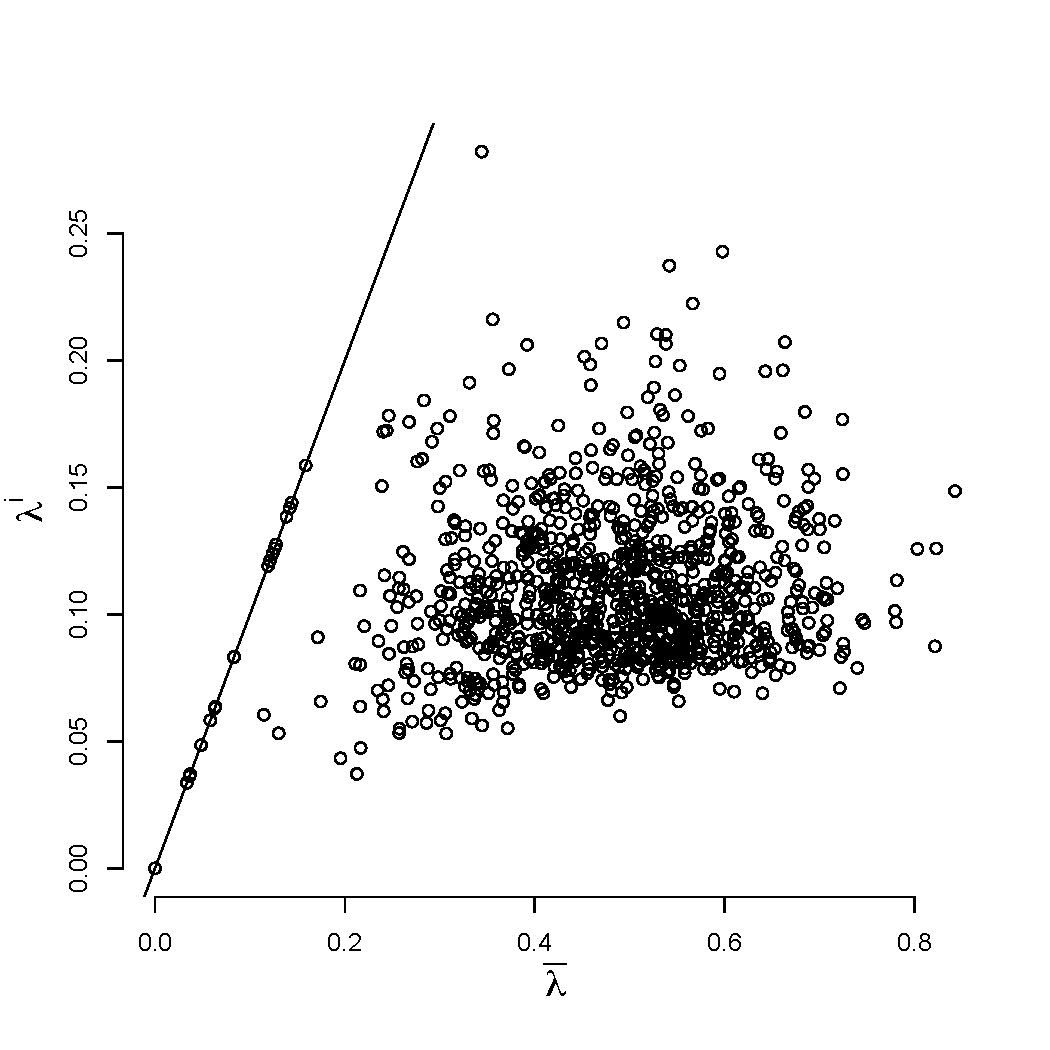
\includegraphics[width=.5\textwidth]{eigenvalue_comparison.pdf}
\end{center}
\caption{\label{eigenvalue_comparison} Here we plot the smallest eigenvalue $\lambda^i$ of the reduced Laplacian $L^i$ against the smallest eigenvalue $\overline{\lambda}$ of the transformed Laplacian $\overline{L}$, for several different matrices.  We find that $\lambda_i\leq \overline{\lambda}$.}
\end{figure}

In addition to the rate of convergence, the steady state distances from consensus can also be affected by individual-level optimizations.  If an individual is trying to minimize $\lim_{t\to\infty}\delta_j(t),$ he will also presumably minimize $\lim_{t\to\infty}\E[||\delta(t)||]$.  Section \nameref{deviations} shows how both $\lim_{t\to\infty}E[||y(t)||]$ and $\lim_{t\to\infty}E[||\delta(t)||]$ can be calculated from the Laplacian matrix $L$.  We find that $\lim_{t\to\infty}E[||\delta(t)||]\geq \lim_{t\to\infty}E[||y(t)||]$ (Figure \ref{lyap_comparison}).  Therefore, in trying to minimize $\lim_{t\to\infty}E[||\delta(t)||]$, an individual will necessarily minimize $\lim_{t\to\infty}E[||y(t)||]$.

Therefore, while a network's ability to come to consensus may not benefit the individual directly, in trying to gather information from the social network as quickly and reliably as possible, the individual is likely to affect the network in a way that would lead to more robust consensus dynamics.

\begin{figure}
\begin{center}
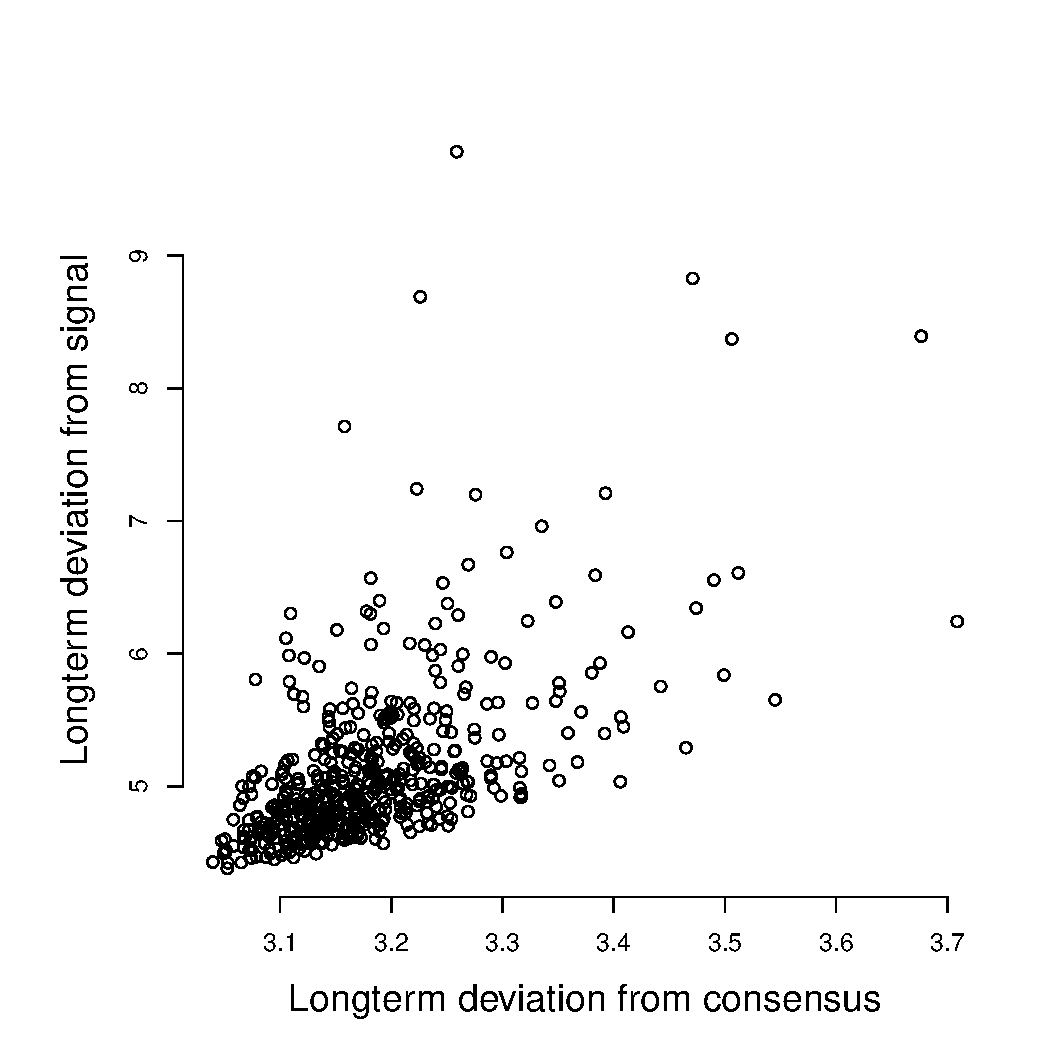
\includegraphics[width=.75\textwidth]{deviations.pdf}
\end{center}
\caption{\label{lyap_comparison} Here we plot the steady state distance from the external signal and the steady state distance from consensus, for many matrices, as calculated in Section \nameref{deviations}.}
\end{figure}

\section{Evolutionarily Stable Information Gathering Strategy?}
Is there an evolutionarily stable information gathering strategy?  For a given network configuration, we can score each node according to how quickly the node would converge to the external signal value.  This is determined by two properties of the reduced laplacian matrix $L^j$.  

As derived above,
$$\dot{\delta}(t)=-L^j\delta(t)+\xi(t).$$
If we ignore noise for the moment, $\delta(t)=e^{-L^jt}\delta(0)$ and the largest eigenvalue of $-L^j$ (and hence the smallest eigenvalue of $L^1$) will determine the rate of convergence for the whole population.   Let $v^j$ be the eigenvector associated with the smallest eigenvalue $\lambda^j$, For sufficiently large $t$, we can approximate $\delta(t)\sim -v^j$ so that $|\delta_i(t)|\sim |v_i^j|$.  Therefore, the absolute value of the $i^{th}$ coordinate of $v^j$ indicates how close to the external signal node $i$ will be in the long run.  These two properties gives a convergence score for each node in the network:
$$e^{-\lambda^j}|v_i^j|.$$
Nodes with smaller convergence scores will gather the external signal more quickly.  Since each node in the network can receive the external signal and the nodes in the network would like to gather that information regardless of the receiver, we will give each node a score 
$$s_i=\langle e^{-\lambda^j}|v_i^j| \rangle_j,$$
where the average is across the different potential receivers $j$.

Before analyzing empirical networks, we'll look at a few idealized networks.  Imagine a cyclical graph of $N$ nodes places in a circle, each of which gathers information from its $k$ nearest neighbors.  We will introduce one invader with a different strategy $k'$ and see whether the natives or the invader get lower convergence scores.  To give a fitness score to the native and invader strategies, we look at the percent decrease in convergence scores between the average native score and the invader score.  Across network sizes there are three general patterns (see Figure \ref{ess_grid}):
\begin{enumerate}
\item if the native strategy is a low number of neighbors, invaders with more neighbors can invade
\item if the native strategy is low, having too many neighbors can be disadvantageous to the invader
\item if the native strategy is high, the dynamics are essentially neutral (except that an invader with a very low strategy can't invade)
\end{enumerate}

The fact that a very high invader strategy does poorly against a very low native strategy highlights the advantages and disadvantages of a high strategy.  If the signal comes to a node far away in the network, the invader can gather that signal more quickly than his poorly connected immediate neighbors.  However, if the signal comes to a node close to the invader, the invader is still collecting information from the nodes from across the circle and thus doesn't converge to the signal as quickly, a cost that is then relayed to his immediate neighbors who gather information from him (Figure \ref{convergence_in_space}).

For a given network size, we would like to know the ESS.  As the dynamics are essentially neutral for high native strategies, there are several high strategies that cannot be invaded by lower strategies but can drift between each other.  We take the minimum such strategy since presumably it's cognitively more parsimonious to attend to fewer rather than to more neighbors.  This ESS rises essentially linearly with the size of the network, so that the optimal number of neighbors is about $2/3$ total network size (Figure \ref{ess_vs_size}).

\begin{figure}
 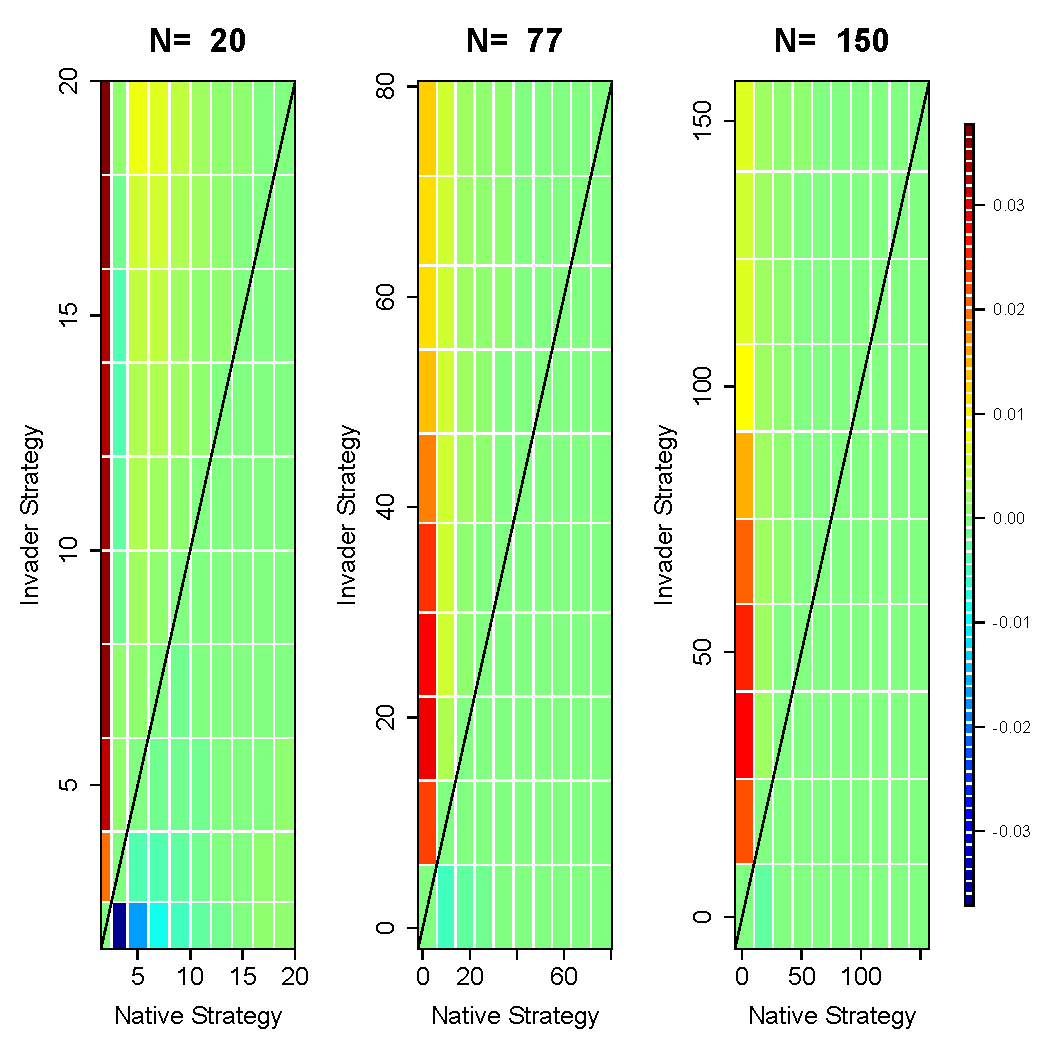
\includegraphics[width=\textwidth]{ess_plot.pdf}
\caption{For various network sizes ($N$), we plot the percent difference in an invader's and a native's convergence score.  When the native strategyis to have few neighbors, an invader with more neighbors does generally (although not monotonically) better.  The landscape is essentially neutral when the native has many neighbors.}
\label{ess_grid}
\end{figure}

\begin{figure}
\begin{center}
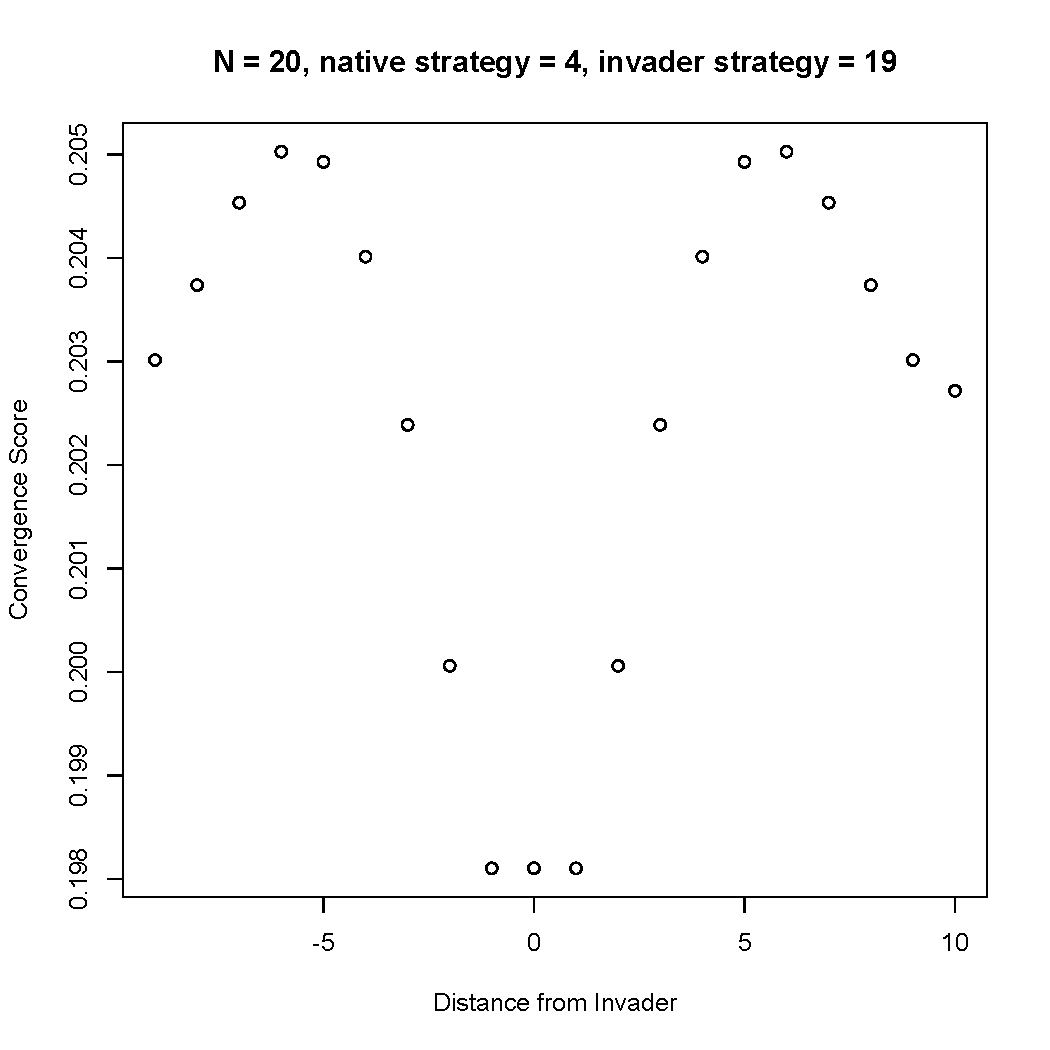
\includegraphics[scale=.5]{how_invader_succeeds.pdf}
\end{center}
\caption{For a network of size $20$ and a native population with a moderate number of neighbors, having too many neighbors cans actually be disadvantageous.  When the receiver is far away from the cheater, the cheater benefits by picking up that long-range signal more quickly than his close-minded neighbors.  However, when the receiver is close to the cheater, the cheater gets a noisy signal from the many sources of information he has.  The immediate neighbors of the cheater on average far worse because they do not benefit from the cheater's long range signal gathering and are harmed by gathering the spurious signal from the cheater when he gets it wrong.}
\label{convergence_in_space}
\end{figure}

\begin{figure}
\begin{center}
\includegraphics[scale=.5]{ess_strategy.pdf}
\end{center}
\caption{For a given network size, we find the minimum neighbor strategy that cannot be invaded.}
\label{ess_vs_size}
\end{figure}




\nocite{*}
\bibliographystyle{plain}
\bibliography{info_evo}

\end{document}


